\documentclass[edeposit,fullpage]{uiucthesis2009}

% Import all packages in Copernicus.
\usepackage[normalem]{ulem}
\usepackage[T1]{fontenc}
\usepackage{textcomp}
\usepackage[utf8]{inputenc}
\usepackage[english]{babel}
\usepackage{array}
\usepackage{tabularx}
\usepackage{graphicx}
\usepackage{overpic}
\usepackage{color}
\usepackage{amssymb}
\usepackage[intlimits,fleqn,tbtags]{amsmath}
\usepackage{amsthm}
\usepackage{url}\urlstyle{same}
\usepackage{accents}
\usepackage{cancel}
\usepackage{multirow}
\usepackage{supertabular}
\usepackage{algorithmic}
\usepackage{float}
\usepackage{algorithm}
\usepackage{caption}
%\usepackage{subfig}
%\usepackage{subfloat}
\usepackage[authoryear,round]{natbib}
\usepackage{rotating}
\usepackage[mathlines,modulo]{lineno}
\usepackage{times}
\usepackage{tikz}
\usepackage{subcaption}  %package for acp paper
\usepackage[version=4]{mhchem} % package for jgr paper
\usepackage{threeparttable} %% package for jgr paper
\usepackage{booktabs}
\usepackage{soul}
\usetikzlibrary{shapes,arrows,chains}

%
\renewcommand{\topfraction}{0.9}	% max fraction of floats at top
\renewcommand{\bottomfraction}{0.8}	% max fraction of floats at bottom

% TODO commands
\newcommand{\jctodo}[1]{{\color{red} #1}}
\newcommand{\jcedits}[1]{{\color{blue} #1}}

% Graphics path
\graphicspath{{./graphics/}}

\pdfinfo{
   /Author (Yu Yao)
   /Title  (Particle-resolved aerosol modeling on the
regional scale -- Insights into importance of capturing
aerosol mixing state)
%   /CreationDate (D:20040502195600)
}

% Custom settings
\renewcommand\thealgorithm{\thechapter.\arabic{algorithm}} 

% Tables
\newcommand\tophline{\hline\noalign{\vspace{1mm}}}
\newcommand\middlehline{\noalign{\vspace{1mm}}\hline\noalign{\vspace{1mm}}}
\newcommand\bottomhline{\noalign{\vspace{1mm}}\hline}
\newcommand\hhline{\noalign{\vspace{1mm}}\hline\noalign{\vspace{1mm}}}

% Need the GMD unit command
\DeclareRobustCommand*\unit[1]
 {\ensuremath{%
   {\thinmuskip3mu\relax
    \def\mu{\text{\textmu}}\def~{\,}%
    \ifx\f@series\testbx\mathbf{#1}\else\mathrm{#1}\fi}}}

    
\newcommand{\kMax}{K_{\textnormal{up}}}
\newcommand{\kMin}{K_{\textnormal{min}}}
\newcommand{\kOver}{K_{\textnormal{over}}}
\newtheorem{theorem}{Theorem}[chapter]
\newtheorem{corollary}[theorem]{Corollary}

% Adjust the length of the table of contents
% List everything (subsubsections)
%\setcounter{tocdepth}{3}
% Chapters and sections only
\setcounter{tocdepth}{1}
\begin{document}

%%%% Title creation
%\nocopyrightpage
\title{Quantifying cloud chemical processes and aerosol optical properties using a particle--resolved model}
\author{Yu Yao}
\department{Atmospheric Sciences}
\phdthesis
\committee{ Professor Nicole Riemer, Chair and Director of Research\\
Professor Sonia Lasher-Trapp \\
Associate Professor Matthew West \\
Dr. Matt Dawson\\}
\maketitle


% Begin front matter
\frontmatter

\begin{abstract}

\end{abstract}

\begin{dedication}
To my family
\end{dedication}

\chapter*{Acknowledgments}


% List of acknowledgements:
%
% Advisors
% Department support, specifically committee.
% Riemer group, specifically Joseph Ching, Laura Fierce.
% CSE fellowship
% DOE ASR grant
% Blue Waters standard acknowledgement

%%%%%%
% Next comes ToC, LoT and LoF
%%%%%%

\tableofcontents
%\listoftables
%\listoffigures

%%%%%%
% Begin the main body
%%%%%%
\mainmatter

%%%%%%%%%%%%%%%%%%%%%%%%%%%%%%%%%%%%%%%%%%%%%%%%%%%%%%%%%%%%%%%%%%%%%%%%
\chapter{Introduction and motivation}
Aerosol particles play an important role in the climate system by directly changing the radiative balance through scattering and absorption radiation, known as aerosol-radiation interactions (ari), or indirectly by changing cloud properties, known as aerosol-cloud interactions (aci). Unlike the greenhouse gases, particles are typically with short lifetime and highly varied in space and time, making the interactions remain the largest uncertainties for future climate prediction. The goal of this dissertation is to help understand the interactions through the aspect of aerosol species. More specially, this project quantifies the changes of aerosol species after cloud processing and how chemical species matter for aerosol optical properties. This chapter gives a general background about aerosol radiative effects, aging processes in cloud and aerosol models with different complexity. 

\section{Aerosol properties}
\label{cha1-1:aerosol-defi}
%Definition of aerosol particles.
Aerosol particles are solid or liquid matter suspended in the air, and it receives tremendous focus recently because of the ongoing COVID-19 pandemic caused by SARS-Cov-2 virus, which is airborne and dominant by aerosol transmission \citep{prather2020reducing,zhang2020identifying, miller2021transmission, greenhalgh2021ten}. Actually, as a part of air pollutants, the health effects of aerosol particles, especially fine particulate matter with diameter less than 2.5~$\rm \mu m$ ($\rm PM_{2.5}$), have been investigated tremendously \citep{bell2007spatial, fann2012estimating}. Around 141\,000 premature death in North America due to cardiopulmonary and lung cancer is associated with $\rm PM_{2.5}$ \citep{anenberg2010estimate}. Besides its crucial impacts on health, aerosol particles can also change weather and climate through interacting with solar radiation and clouds, which still exist large uncertainties to quantify these impacts \citep{IPCC_CHAPTER7, seinfeld2016improving, fan2016review, bellouin2020bounding}. 

Aerosol particles can be directly emitted from different sources, or formed secondary from gas precursors. The major components of particles are inorganic species, carbonaceous species, sea salt and mineral dust. These species can originate from natural or anthropogenic sources, and the formation pathways are also varied. Sea salt particles are generated primarily over ocean region through mechanical processes and strongly depend on wind speed \citep{jaegle2011global, monahan1986model}. Dust is another primary natural species originated from desert regions and can affect remotely through long-range transport \citep{van2018mysterious,yu2021observation}. The dominant pathway of inorganic species are secondary through either nucleation or gas-to-particle partitioning. For example, sulfate can form through nucleation of sulfuric acid with the presence of water vapor \citep{sipila2010role}, and it can also be produced through oxidation of $\rm SO_2$ by OH in gas phase or $\rm H_2O_2$ and $\rm O_3$ in aqueous phase \citep{shao2019heterogeneous, zheng2020multiphase}. Primary and secondary are both prevalent pathways for organics formation. Black carbon (BC) and primary organic aerosol (POA) are usually co-emitted from combustion of fossil fuel and biofuel \citep{bond2007historical}. Formation of secondary organic aerosol (SOA) involves partitioning with semivolatile species, oligomerization and aqueous chemistry \citep{zhu2017mechanism, lim2010aqueous, griffin2013sources, mcneill2015aqueous}.
%Aerosol particles diameters range from several nanometers to over 10 $\rm \mu m$.  

Aerosol diameters vary from molecular aggregates with several nanometers to dust particles with several micrometers \citep{MCMURRY200320}. It is common to represent aerosol size distribution by three modes: Nuclei mode (0.01 -- 0.1 $\rm \mu m$), accumulation mode (0.1 -- 2 $\rm \mu m$) and coarse mode (2 -- 10 $ \rm \mu m$). Nuclei-mode particles are commonly observed near combustion sources, especially roadside atmosphere, and characterized by high number concentration, which can engender efficient coagulation and result in short lifetime for these particles \citep{fushimi2008atmospheric}. Accumulation-mode particles contain most of the secondary species, such as sulfate, nitrate and organics \citep{zhang2005time}, and they can also be produced from coagulation of the nuclei-mode particles. As for coarse-mode particles, it is hard to grow such large by coagulation alone between small particles \citep{friedlander1991scavenging, lee2005size}. They are mostly originated from natural sources and produced by mechanical forces. They suspended shortly in the air due to rapid gravitational settling. 

\section{Aerosol climate forcing}
\label{cha1-2:aerosl-climate}
Aerosol can change radiation balance of Earth system through direct interactions with shortwave and longwave radiation. Globally, average net effects change of direct aerosol effective radiative forcing between 1750 and 2005 is estimated to be $-0.45$ $\rm W$ $\rm m^{-2}$, as shown in Figure~\ref{fig:chap1-aerosol-climate}. Estimation of the effects relies on the properties of aerosol population, such as size and chemical components, and the wide variety of aerosol particles at different regions leads to spatial variation of this effect. For example, directive radiative forcing over top of atmosphere over Africa is around $-12$ $\rm W$ $\rm m^{-2}$, while it can reach +$30$ $\rm W$ $\rm m^{-2}$ over polluted Indo-Gangetic Plains \citep{subba2020recent}. 

\begin{figure}
	\centering
	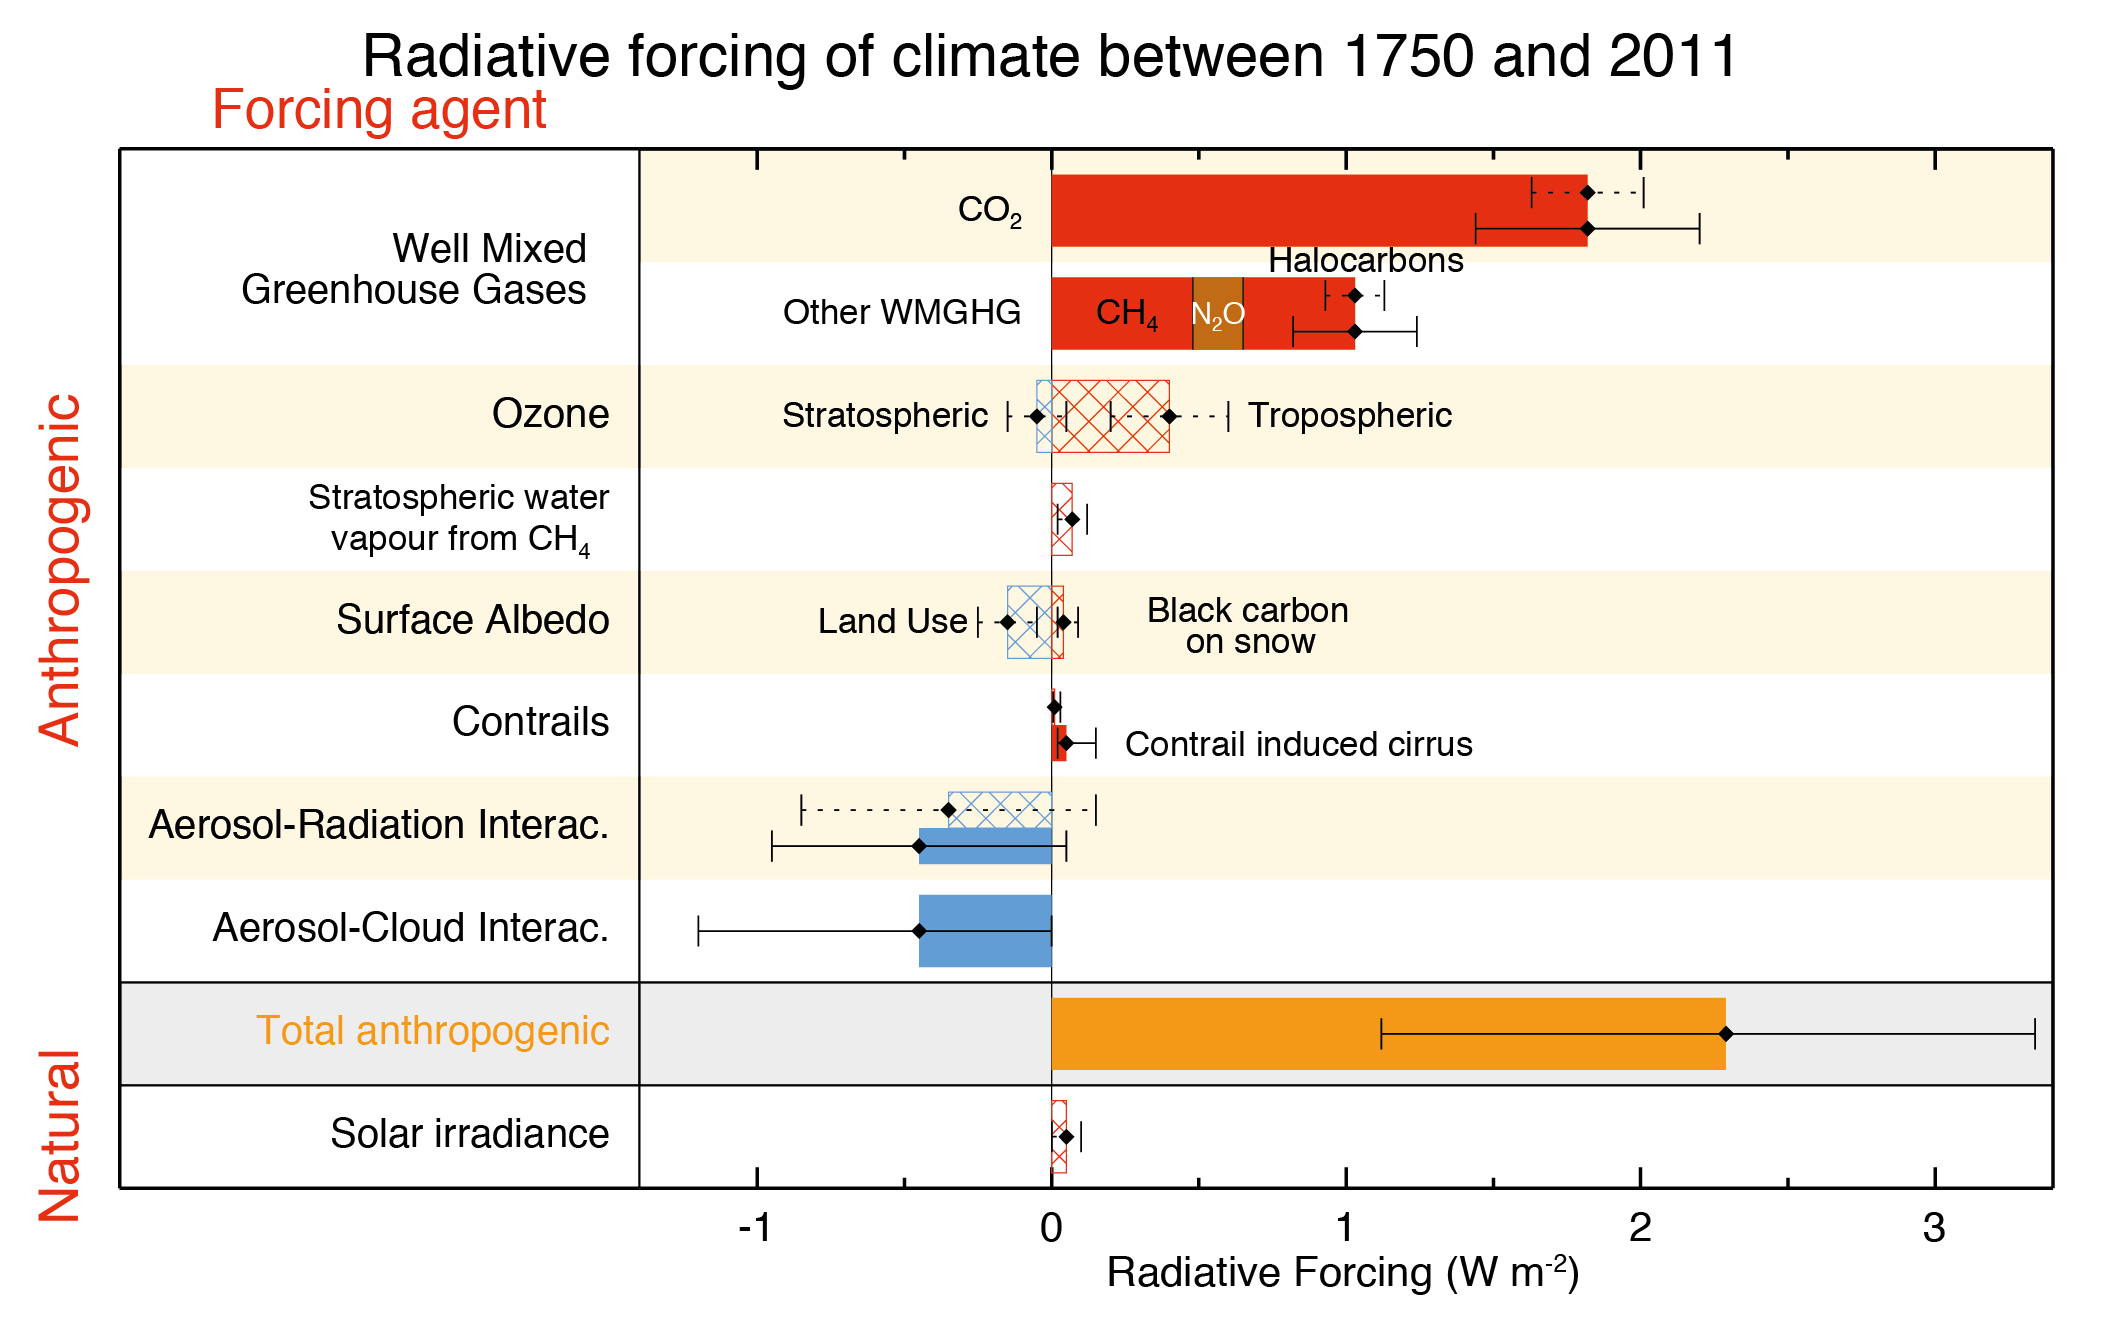
\includegraphics[scale=0.80]{chap1_figs/thesis_chap1_fig1.jpeg}
	\caption{Radiative forcing estimation of different agents between 1750 and 2011, adapted from \cite{IPCC_CHAPTER8}.}
	\label{fig:chap1-aerosol-climate}
\end{figure}

As a condensation nuclei, aerosol particles can also indirectly affect climate through interactions with cloud, and the estimated effective radiative forcing from this interaction is $-0.45$ (Figure~\ref{fig:chap1-aerosol-climate}). There are many processes involved in the interactions and they can be illustrated by two main effects: cloud albedo and lifetime effects. Cloud albedo effects, first proposed by \citet{twomey1977influence}, describe the changes of cloud number concentration and surface area at environment with different aerosol loading, and it had been supported by ambient observations. \citet{kaufman2005effect}, by analyzing satellite observation over Atlantic ocean, found liquid clouds coverage in the polluted environment is higher by 0.2$-$0.4 than clean environment, and with smaller droplets. Field observations also confirme that more cloud condensation nuclei (CCN) generate more cloud droplets with smaller sizes in liquid clouds \citep{jia2019distinct,kleinman2012aerosol}. Cloud lifetime effect is the mechanism that the increase of aerosol number concentration will result in smaller cloud droplets and inhibiting precipitation development. Considering smaller droplets are hard to trigger coagulation coalescence, this effect is theoretically reasonable if only considering precipitation initiation. However, several observations and model studies suggested this effect can be problematic under different cloud environment due to the unclear relation between initial cloud droplet size and evolving precipitation efficiency \citep{stevens2009untangling}. 
% May do not need to mention this because we are not going to talk about it. 
%The physical understanding of interactions with liquid cloud improves substantially in past decades, but the interactions with ice and mix-phased clouds is still poor constrained. 

As we can see from figure~\ref{fig:chap1-aerosol-climate}, there still exists large discrepancies in the aerosol related radiative forcing amplitudes among different models. For radiative forcing from aerosol radiation interaction, the estimated 5 to 95\% confidence ranges from $- 0.95$ to $+ 0.05$ $\rm W$ $\rm m^{-2}$, while the range is from $-1.2$ to $0.0$ $\rm W$ $\rm m^{-2}$ for aerosol-cloud interaction. The sources of the uncertainty lie in the fact that there are multiple scale processes are involved, from particles as small as 10~nm to 1000~km stracumulus clouds. Many processes are still unclear, such as aerosol interaction with mix-phase and ice clouds, simple parameterization schemes are applied to describe these processes in the models. Even for those processes that are well-contrained, it is challenging to incorporate all these processes in a single model \citep{seinfeld2016improving,bellouin2020bounding}. By interacting with electromagnetic radiation, and acting as an nuclei for cloud formation, particles are fundamental for quantifying these forcing and accurate description of aerosols can help reduce the model uncertainly. 

\section{Aerosol mixing state}
Mixing state, which defines the distribution of chemical species among the particle population, is an appropriate concept for describing aerosols \citep{winkler1973growth}. There are two mixing state extremes for an aerosol population:internal mixture and external mixture. With internal mixture, particles are assumed to have the same components and the same mass fraction of the species. While for a population with external mixture, all particles only contain single specie and they are externally mixed. These two extremes are rarely observed in real environment, and particles are common in the intermediate mixing state. In other words, particles can contain different species and mass in the population. Figure~\ref{fig:chap1-mixing} shows the transmission electron microscopy (TEM) images of carbonaceous-bearing particles collected in urban Shanghai in 2010. Particles are the mixture of different species. Some are mixture of two species (a, b, c), others are mixture of more than three species (f, g, h, i).  

\begin{figure}
	\centering
	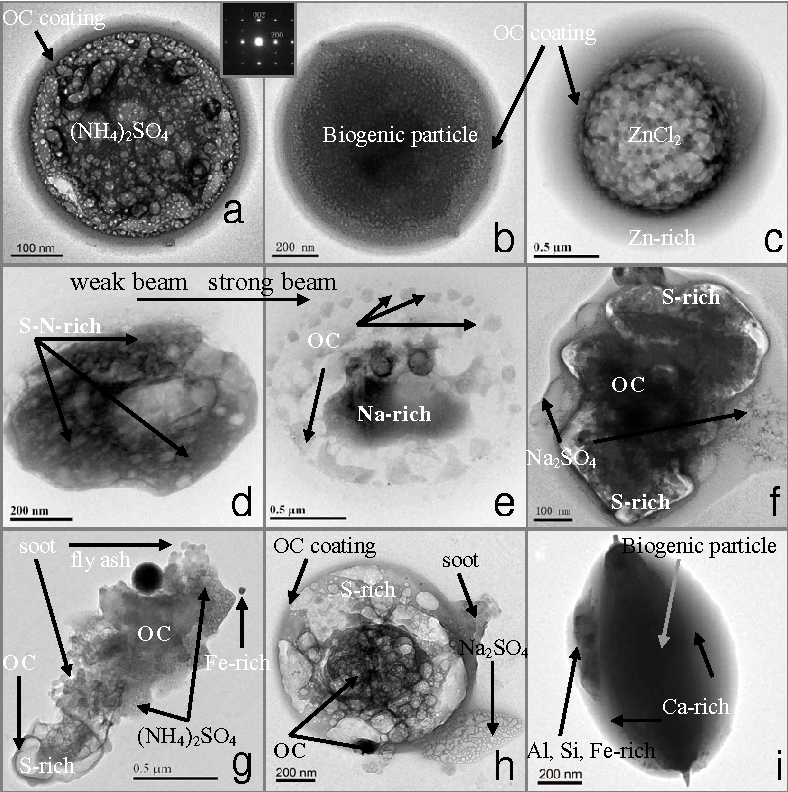
\includegraphics[scale=0.40]{chap1_figs/thesis_chap1_fig2.png}
	\caption{TEM images of C-bearing particles collected from urban Shanghai, adapted from \cite{fu2012morphology}.}
	\label{fig:chap1-mixing}
\end{figure}

Since hygroscopicity and optical properties are varied in different species, which are important factors for droplets formation and radiative behaviour, aerosol population with different mixing state will produce varied climate-related properties, as illustrated in figure~\ref{fig:chap1-chi-climate}. For populations with the same amount of ammonium sulfate and organic, but the species are distributed differently among the particles, as figure~\ref{fig:chap1-chi-climate}(a) shows. In the population with internal mixture, all the particles have the same amount of ammonium sulfate and organic. But for the population with external mixture, half contains sulfate and half contains organic. But in the real world, these two species can randomly distribute among the particles. If these three populations are exposed at the same supersaturation environment (ss = 0.3\%), the number of activated particles is varied. All the particles are activated in the population with internal mixture, and only half are activated in the externally mixed population. The activated particles number in real world case are between these two extremes. We can apply the same strategy for explanation of aerosol optical properties. Figure~\ref{fig:chap1-chi-climate}(b) shows the populations with the same amount of absorbing species (BC) and non-absorbing species ($\rm NH_4HSO_4$), but with different mixing state. As a result, the optical properties, including single scattering albedo (SSA), ensemble scattering coefficeints ($\beta_{\rm abs}$), ensemble absorbing coefficients ($\beta_{\rm abs}$) and asysmetry ($g$), are varied in the populations and can lead to different radiative forcing effects.

\begin{figure}
	\centering
	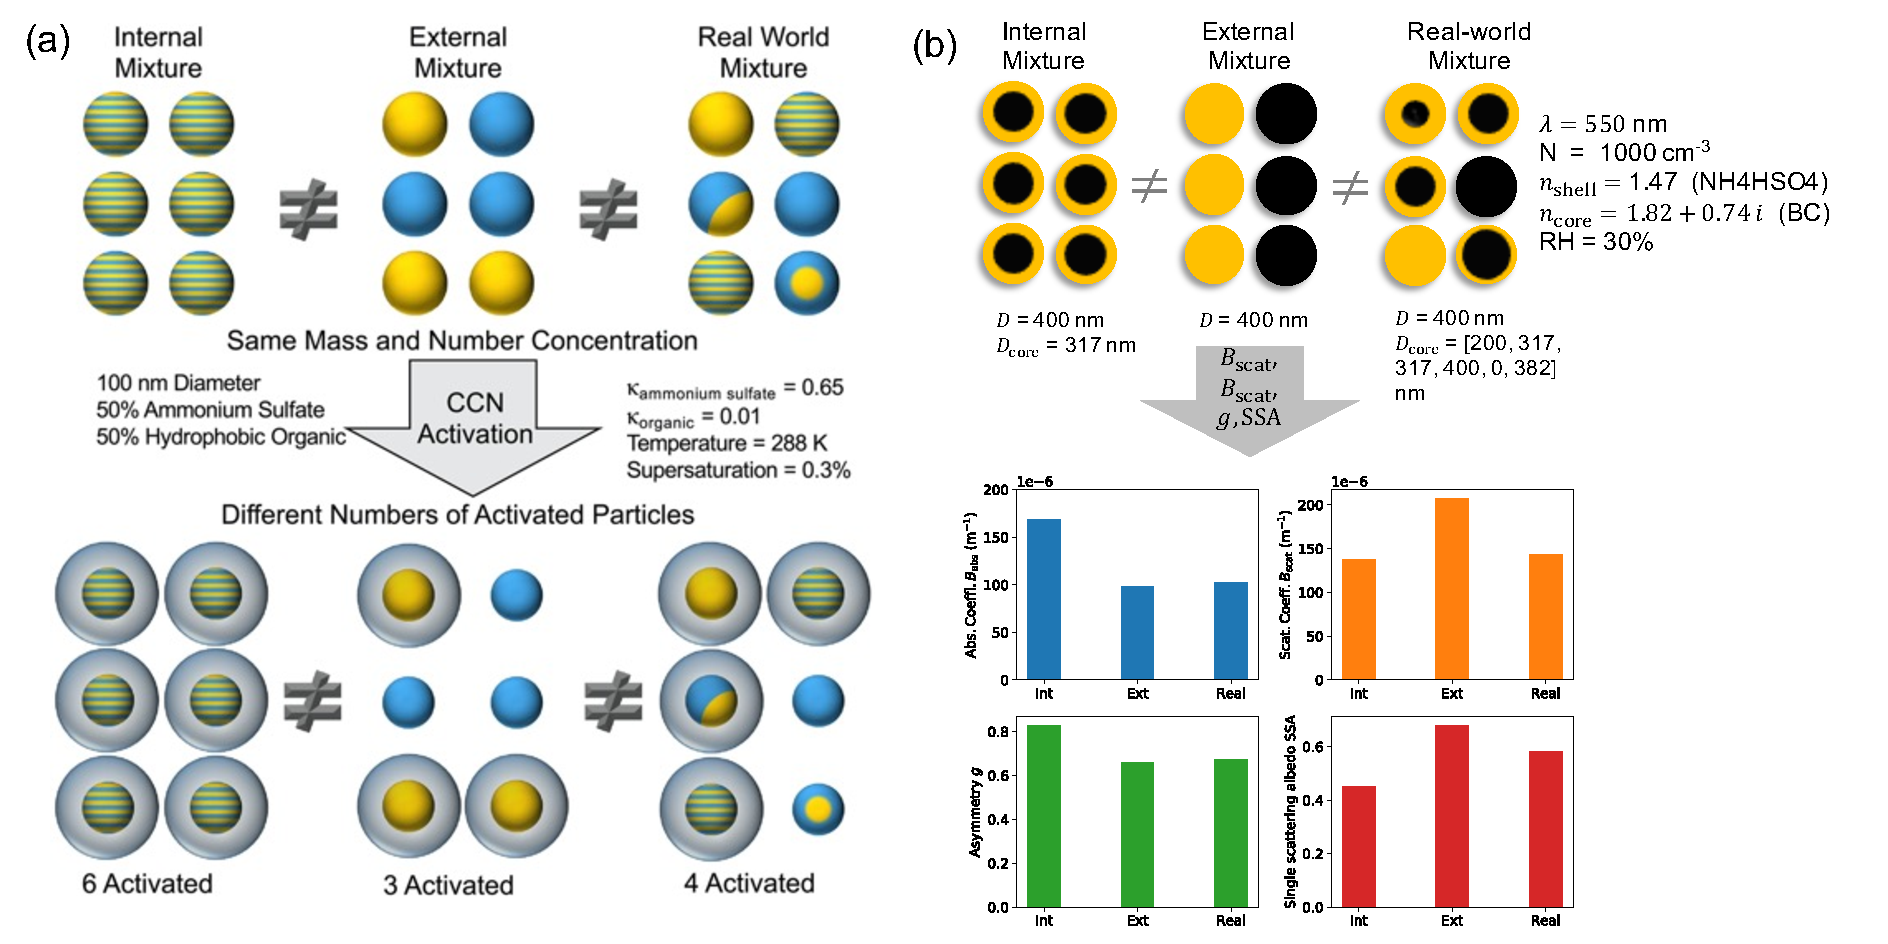
\includegraphics[scale=0.60]{chap1_figs/thesis_chap1_fig3.pdf}
	\caption{Aerosol mixing state effects on (a) activation ability and (b) optical values. (a) is adapted from \cite{Riemer2019}.}
	\label{fig:chap1-chi-climate}
\end{figure}

The effects of mixing state on aerosol activation potential can be investigated through closure study. Aerosol/CCN closure study is conducted by comparing the observed and predicted CCN concentration at the same supersaturation level. The prediction is made by applying K$\ddot{\rm o}$hler theory, using the measured dry particle size distributions and components information as input, with assumptions in mixing state to examine its effects.  \citet{broekhuizen2006closure} performed the closure study for aerosol samples from downtown Toronto at 0.58\% supersaturation, and they found the internal mixture assumptions overpredicted the CCN concentrations by 0.12$\pm$0.05. Using the CCN sampled from 2010 CalNex field campaign, \citet{moore2012hygroscopicity} also found internal mixture resulted in 30--75\% overprediction of CCN concentration. 

As for the effects on aerosol optical properties, aerosol mixing state affect its absorption or scattering abilities from the following aspects. First, as a major factor in determining aerosol optical properties, complex refractive index is distinctive for each species. Inorganic species only have real part of the index and have cooling effects. It is more complicated when refer to organic species, which are also initially treated as cooling species, and the warming effects and the value of imaginary part of the index of the organic species have received more attention recently \citep{corbin2018brown, Esteve2014, cappa2019light}. Second, in a humidified environment, water update of a particle depends strongly on its composition because of varied hygroscopicity of the species, which is important for scattering \citep{MichelFlores2012, Zieger2013, Titos2014, Titos2016}. Studies showed, compared with dry environment, scattering ability can be enhanced by 1.6 at the environment with RH of 85\% \citep{Burgos2020}. At last, the distribution of the diverse species in a particle is important in determining optical values. For particles with no strong absorber, i.e. BC, volume-mixing rule can be used to calculate the refractive index and when BC is contained in the particle, core-shell configuration is proved to bBurgos2020e more accurate \citep{Bond2006}. The absorption enhancement of BC-contained particles due to its surrounding coatings are widely investigated \citep{Moffet2009,Liu2017, wu2020light}, and distribution of the non-absorbing species are found to be the main sources for the discrepancies between the simulated and observed optical values \citep{Fierce2016, Fierce2020}.

\section{Aerosol mixing state evolution}  
Aerosol mixing evolution is a complex procedure and several processes are involved. At the time of particles emitted from the sources, aerosol population can already be the mixture of different species. For example, BC emitted from diesel vehicles are mixed with organics and sulfate, and the sea-spray aerosols are the mixture of sodium chloride and organics \citep{cheung2010emissions, kirpes2018secondary}. Once emitted, mixing state can further be modified by condensation of low-volatility compounds, such as the sulfate produced from oxidation of $\rm SO_2$ by OH in gas-phase. Heterogeneous reactions between gas-phase reactants and condensed-phase surface can be faster than reactions in gas-phase, and one important reaction is the ozone depletion by chlorine radials produced from heterogeneous reactions between chlorofluorocarbons and polar cloud surface \citep{davies2018heterogeneous}. Coagulation between particles is an efficient process in changing particle number concentration and Brownian coagulation had been proved to the main reason for the 
rapid evolution of soot particle size distribution near a highway emitting point \citep{jacobson2004evolution}. The processes outlined above are for the cloud-free environment, however, since the global cloud coverage is more than 0.6 on average \citep{stubenrauch2013assessment}, evolution in clouds is also an important course during the lifetime of aerosol populations.

Figure~\ref{fig:chap1-aq-proc} shows the chemical and physical processes particles experience in an aqueous environment. When the atmosphere reach supersaturated, particles with critical supersaturation lower than the environment supersaturation are activated as cloud droplets and undergo nucleation scavenging. For these activated particles, the absorbed water facilitates the aqueous chemical reactions. Gas species dissolve in the cloud, and if both liquid and ice phase exist in the cloud, species partition between different phase occurs and the retention coefficients in liquid phase are varied. When cloud droplets grow to rain droplets, they fall out and precipitate. During the falling out procedure, some small interstial particles are collected by these large droplets and impaction scavenging occurs. For clouds with strong convection, gas and particle species are vertically redistributed by convective transport. 

\begin{figure}
	\centering
	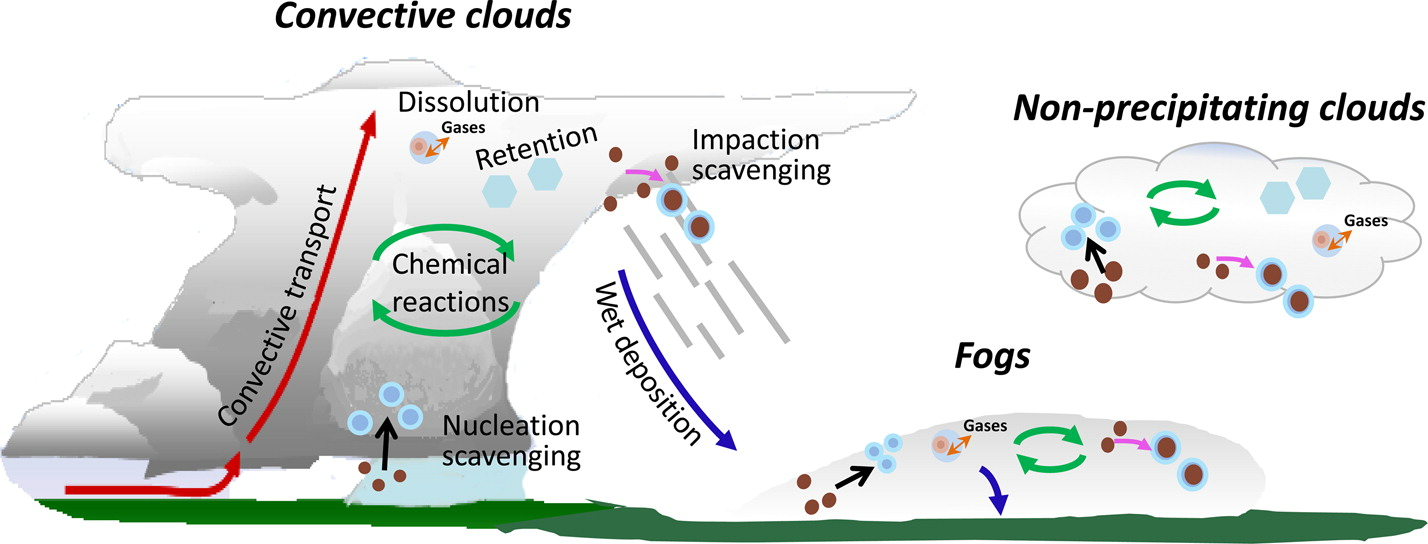
\includegraphics[scale=1.0]{chap1_figs/thesis_chap1_fig4.jpeg}
	\caption{Processes schematic invovled in fogs and clouds, adapted from \cite{ervens2015modeling}.}
	\label{fig:chap1-aq-proc}
\end{figure}

Aqueous environment provides an efficient medium for sulfate formation. Globally, more than 50\% of sulfate forms through in-cloud oxidation and the formation rates of aqueous reactions, $\rm SO_2$ oxidation by $\rm H_2O_2$ and $\rm O_3$, are more effective than through OH oxidation in gas phase \citep{kreidenweis2003modification, rasch2000description}. Other aqueous sulfate formation mechanisms, such as the reactions catalyzed by Transition Metal Ions (TMI), can also be important and it is confirmed to be the dominant pathway for the sulfate formation in the samples collected during HCCT-2010 field campaign \citep{harris2012sulfur, harris2013enhanced}. 

%Reaction rates of aqueous processes rely on cloud properties and the importance of different pathways differs at various cloud types.  \citet{straub2007chemical}, analyzing the marine stratocumulus cloud samples collected over eastern Pacific Ocean during DYCOMS-II field campaign, found $\rm SO_2$ oxidized by $\rm H_2O_2$ is the dominant reaction for sulfate production.
Recently, more emphasis transfers to the role of aqueous reactions for SOA formation. Globally, SOA produced from aqueous pathway can reach to 20--30 Tg·$\rm yr^{-1}$. Glyoxal, methylglyoxal, glycolaldehyde and acetic acid can act as the precursors for aqueous SOA \citep{liu2012global}. As for the oxidants, besides hydroxyl radical, which is the dominant oxidant for SOA formation at gas phase, aqueous environment can provide several other efficient oxidants, such as peroxyl radicals, peroxides and triplet excited states of organic compounds ($^{3}\textrm{C}^*$) \citep{mcneill2015aqueous, ervens2011secondary}. Using simulated sunlight UV, \citet{smith2014secondary} found phenols can be rapidly oxidized by $^{3}\textrm{C}^*$ to produce low-volatility SOA . 

Aerosol size distribution evolves after the formation of aqueous inorgaincs and organics. Hoppel minima, which describes the CCN concentration gap between two particle distribution modes peak at 0.02--0.03 and 0.08-0.15~$\rm \mu m$ respectively,  was found by \citet{hoppel1986effect} when analyzing the particles processed by nonprecipitation clouds. This phenomena has further been observed for the particles at different region, such as VOCALS campaign over west Chilean coast at Arica and MASE experiment over central California coast \citep{kleinman2012aerosol, hudson2015cloud}. Besides the aqueous aerosol formation, particle size distribution also changes due to coagulation between interstitial particles and cloud droplets. \citet{pierce2015importance} found this process can reduce total particle number concentration by 10--15\% globally.  
\section{Aerosol modeling approaches}
Application of diversified measuring techniques help advance our understanding of aerosol particles, and we know the observed particles are the consequence of multiple processes. By using numerical models, we can distinguish the underlining physical and chemical laws leading to the complexity of aerosol behaviour, and predict what will happen if certain processes change. Considering the wide ranges of species types and sizes for an aerosol population, it is hard for a single model to represent the complete processes the population can experience during its lifetime, from emission to deposition, and balance need to be reached between model accuracy and computational efficiency. This section summaries the current aerosol modeling approaches from simplistic bulk methods used in global models to comprehensive particle-resolved models used in box model, and we will focus on how these models deal with aerosol mixing state and its implication for aerosol related climate properties. 

\subsection{Bulk models}
The simplest aerosol modeling approach is using bulk method. Aerosol population are represented by several common species mass concentration, including sulfate, nitrate, BC, organics, dust and sea salt, and these species are treated as external mixtures in the bulk without detail information about how the species mixed with each other. Rather than tracking the aerosol evolution through microphysical processes, this approach prescribes the aerosol size distribution from climatology data. This approach is computationally efficient and applied by several global models, such as GOCART \citep{chin2000atmospheric} and TM5 \citep{vignati2010sources}. 

\subsection{Modal models}
A more advanced approach is representing the aerosol populations by several modes. Just as shown in figure~\ref{fig:chap1-aerosol-model}(a), modal model tracks the size distribution evolution of the modes. Each mode can contain a variety of species and mixing state of the population are represented by the modes. But inside each mode, all species are still assumed to internally mixed. Considering the wide range of particle diameters, it is convenient to use lognormal function to represent the number distribution of each mode as follows:
\begin{equation}
\centering
    n({\rm log}D_p) = \sum_{i=1}^{m}\frac{N_i}{\sqrt{2\pi}{\rm log}\sigma_i}{\rm exp}(-\frac{({\rm log}D-{\rm log}{\overline{D}_i})^2}{2{\rm log}^2\sigma_i}),
\end{equation}
where $m$ is the mode number, $N_i$ is the number concentration of mode $i$, $\overline{D}_{i}$ and $\sigma_i$ are for the mean diameter and standard deviation of the distribution respectively. The number of modes can be varied among the models. Aitken, accumulation and coarse modes are the essential three modes used in global models, such as MADE used in ECHAM4 global climate model and CMAQ regional chemistry model \citep{lauer2005simulating, binkowski2003models}. Other models apply additional modes to better represent the hydrophilic and hydrophobic species. For example, MAM7 used in CAM5 global model apply additional primary carbonaceous mode, including emitted primary organic matter and BC, which has lower hygroscopicity than accumulation mode \citep{liu2012toward}. For the three parameters used to describe the lognormal distribution, standard deviation of each mode is prescribed, and number concentration and mean diameter change as particles evolve.

\begin{figure}
	\centering
	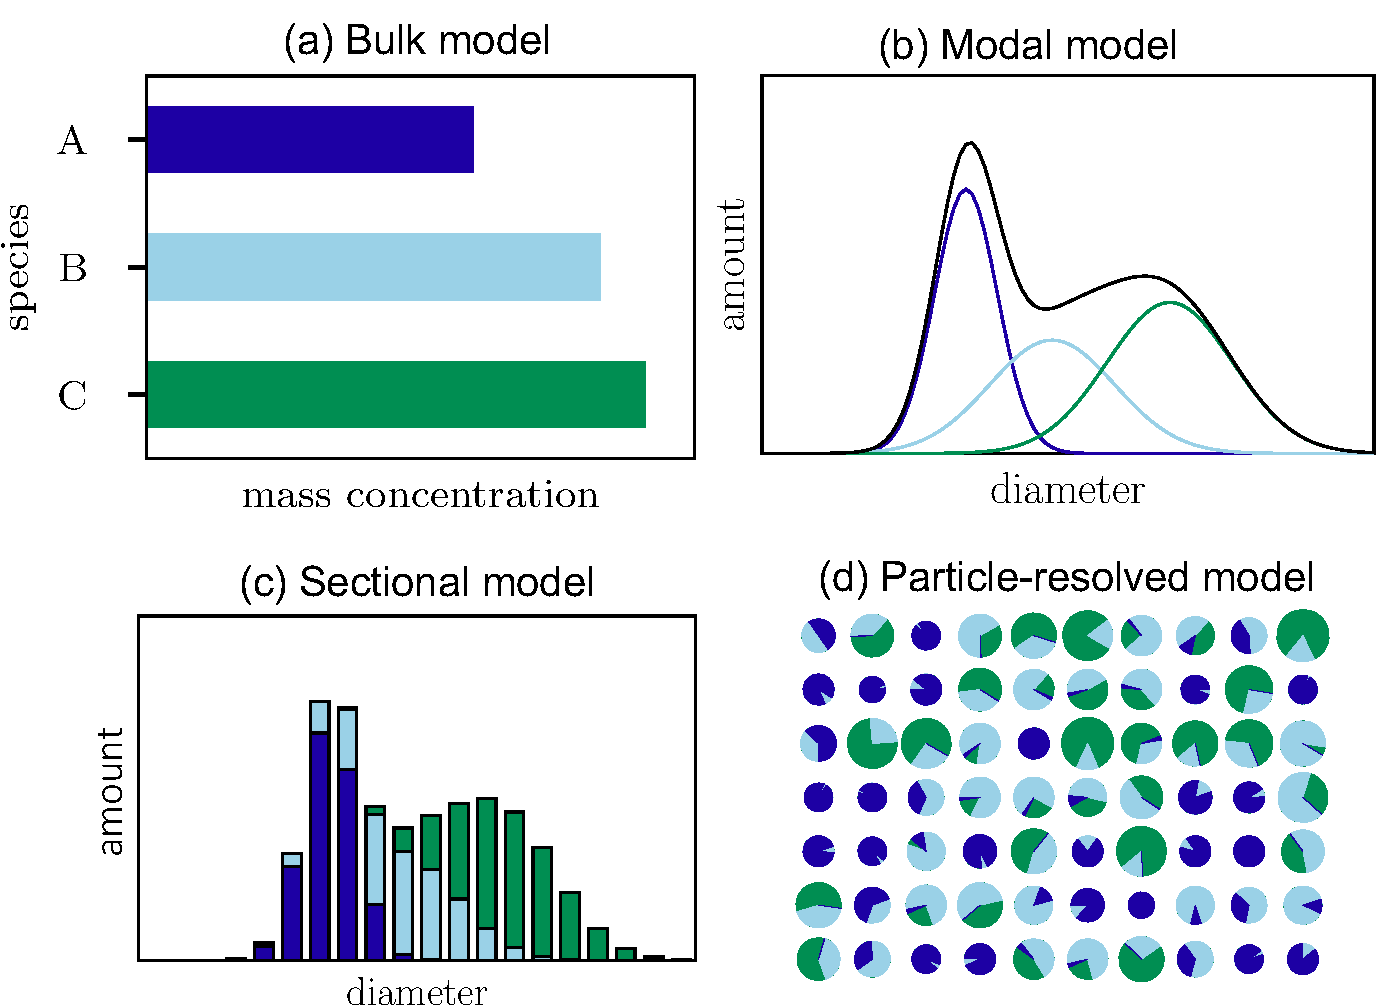
\includegraphics[scale=0.5]{chap1_figs/thesis_chap1_fig5.pdf}
	\caption{Aerosol numerical approaches:(a) Modal model, (b) Section model, and (c) Particle-resolved model}
	\label{fig:chap1-aerosol-model}
\end{figure}

\subsection{Sectional models}
Similar to modal methods, sectional aerosol models are also distribution-based. Instead of tracking the population by different modes, this approach discrete the population to a certain number of size bins and then track the changes in each bin, as illustrated in figure~\ref{fig:chap1-aerosol-model}(b). Particles are internally mixed within the bins and externally mixed between the bins. These aerosol modules are widely applied to large-scale models. For example, MOSAIC with flexible size bin numbers is extensively used in WRF-Chem and proved to capture the summer particulate matter distribution well over Houston region \citep{zaveri2008model,fast2006evolution}. Initially with 30 bins resolving particles with diameter between 0.01 and 10 $\rm \mu m$, TOMAS sectional model is applied to several global chemistry models, such as GEOS-Chem, and improved its ability in simulating aerosol optical properties recently through more detail mixing state representation of BC-contained particles \citep{adams2002predicting,pierce2013weak,kodros2018size}.

Most sectional models apply univariate distribution of aerosol properties with assumptions used to describe aerosol mixing state in each bin, and more advanced schemes have been developed to incorporate more particle details inside the size bin, especially BC mass fraction of the particles. Based on Model of Aerosol Dynamics, Reaction, Ionization, and Dissolution (MADRID) module, \citet{oshima2009aging} developed a two-dimensional sectional scheme MADRID-BC by adding another dimension for BC mass fraction and tracking the fraction changes due to condensation/evaporation processes. Through developing MOSAIC-MIX, \citet{ching2016three} further extended the sectional model representation by incorporating another dimension for hygroscopicity, and coagulation process had been added to evaluate its effects on BC mixing state. 

\subsection{Particle-resolved models}
Even though modal and sectional models provide better representation of particle distribution than bulk models, aerosol mixing state are still simplified by using internal or external assumptions. A more advanced representation of aerosol mixing state is particle-resolved method, as illustrated in  figure~\ref{fig:chap1-aerosol-model}(c). Rather than tracking particles by distribution, particle-resolved model applies Langrangian method to track the particles individually and with no assumptions about the components of the particle. Specifically, each particle is represented by a $A$-dimensional vector, where $A$ is the total species number. The first particle-resolved aerosol model was developed by \citet{Riemer2009} and it was coupled with MOSAIC module to include gas-particle partitioning and gas chemistry processes. The model was applied to investigate the aging process of BC-contained particles in a urban plume environment and the evolution of ship plume particles \citep{tian2014modeling, Ching2016}. Recently, PartMC-MOSAIC had been further coupled with WRF-chem to track particle evolution at large-scale domain \citep{curtis2017single}. 

\section{Models for aqueous chemistry simulation }
One of the topics for the thesis is to investigate the interactions between aerosol mixing state and aqueous chemistry. The previous section discussed the different approaches to simulate aerosol mixing state, and it is different story when comes to incorporating aqueous mechanism for models. From particle activation at manometer scale to stratocumulus structure over thousand kilometers, the magnitude of cloud processes involves around $10^{14}$ orders and it is hard for a single model to incorporate all the related processes. Models with aqueous processes can be divided into two groups: process model with explicit aerosol microphysics and complex aqueous chemical mechanisms, and large-scale model with simplified representation of cloud properties and processes. 

For process models, such as box and parcel models, aerosol microphysics are well-resolved. Droplet activation is explicitly described by using K$\rm \ddot{o}$hler theory. Specifically, particles with critical supersaturation lower than maximum supersaturation reached in the environment are activated as droplets \citep{rothenberg2016metamodeling, ching2012impacts}. Detail aqueous chemistry processes can be incorporated to these cloud parcel models. An example is the cloud parcel model SPACCIM coupled with detail aqueous scheme CAPRAM (492 species and 1087 reactions in version 3.0), and it had been testified using FEBUKO observation data \citep{wolke2005spaccim}. Since particle size distributions are commonly described in process models, the modification of particles after cloud processes can also be captured. The limitation of these models is lacking the interactions with cloud macro dynamics.

It is hard to include such detail information for global models with coarse grids. Rather than resolving cloud microphysics through explicit equations, cloud properties are described by using cloud fraction, with other diagnosed meterological parameters, for each grid. Cloud droplet sizes are assumed to be certain sizes. For example, ECHAM5-HAM assumed two bins for the cloud droplets: one bin for particles with lower ion concentration and the other bin for high ion concentration. As for the effects of cloud droplets representation on cloud chemistry, \citet{barth2006importance}, by camparing sectional and single-size droplet parcel model, found simplified cloud droplet size representation will lead to biases in simulated formic acid and formaldehyde concentration. Simplified aqueous mechanisms are also used and the acidity, which is an important factor for aqueous chemistry, are fixed at constant value. For example, GEOS-Chem used a pH of 4.5 for $\rm SO_2$ oxidation reaction by $\rm O_3$\citep{park2004natural}. Furthermore, assumptions should be made to consider the redistribution of species produced from aqueous reactions. For example, in CMAQ, all the non-volatile aqueous-formed species are added to accumulation mode after cloud dissipates \citep{binkowski2003models, fahey2017framework}. 
 
%\begin{table}
%\setlength\extrarowheight{5pt}
%\centering
%\caption{Overview of acidity, mixing state and optical calculation treatment in different models}
%\label{tab:input}
%\begin{tabular}{ c c c c c}
%	\hline
%	Model acronym  & Model scale &  pH  &  mixing state & Optical calculation  \\
%	\hline
%    CMAQ & Regional & Equilibrium pH & Internal mixture in each mode & \\
%    WRF-Chem (MOSAIC) & Regional  & Equilibrium pH & Internal mixture in each bin &\\
%    GEOS-Chem (TOMAS) & Global & fixed pH at 4.5 & Internal mixture in each bin & \\
%    MOZART & Global & pH based on charge balance &  & \\
%    ECHAM5-HAM & Global & 
%    \begin{tabular}{@{}c@{}}pH based on initial aerosol \\ at small and large droplets\end{tabular} & Internal mixture in each mode & \\
%    PartMC-MOSAIC & 0-D & \begin{tabular}{@{}c@{}}pH based on detailed \\ mechanism at CAPRAM 2.4\end{tabular} & particle-resolved & \\
%	\hline
%   \end{tabular}
% \end{table}
\section{Research questions and thesis organization}
Aerosol particles affect climate forcing through directly altering radiation and indirectly interactions with clouds. These effects are dependent on particle chemical species, in other words, the chemical species mixing state of the aerosol population. Overall objective of this dissertation is to disentangle the complex interactions between aerosol mixing state and its climate effects . 

The following scientific questions will be addressed: (1) At what aqueous environment will TMI-catalyzed oxidation reactions be efficient for sulfate formation? (2) To what extent does cloud processing change the aerosol mixing state of the population that entered the cloud? 
(3) How does this change the cloud condensation number concentration and optical properties? (4) What is the role of coagulation between the interstitial particles and cloud droplets for mixing state of the aerosol?  (5) What is the error in aerosol optical properties introduced by internal mixture assumptions used in sectional models? (6) Will the optical properties error sectional models amplified or dampen at humidified environment? 

Chapter 2 answers the first question by applying coupling particle-resolved model PartMC-MOSAIC with aqueous mechanism CAPRAM. This work designed ensemble cases with three levels of initial gas mixing ratio and temperature lapse rates to find out the cases with efficient sulfate production rates oxidized by TMI. The findings will be concluded in the preparing paper ``Sensitivity of sulfate in-cloud chemistry to aerosol acidity variability and mixing state'' for \textit{Aerosol Science and Technology}. 

Chapter 3 investigates the cloud processing effects on aerosol properties. In this work, we used a typical urban plume particle population to experience four cloud cycles to determine the changes of aerosol mixing state and quantify the changes of aerosol microphysical and optical properties after cloud evaporates. Another simulation is conducted to identify the role of coagulation between cloud droplets and interstitial particles. This chapter will answer questions 2--4. A paper entitled ``The impacts of cloud processing on resuspended aerosol particles after cloud evaporation'', which is in review for \textit{JOURNAL OF GEOPHYSICAL RESEARCH-ATMOSPHERES}, summaries the results on the changes of aerosol microphysical properties after cloud processing. Another paper, which is entitled with ``Quantifying the Effects of Cloud Processing on Aerosol Optical Properties Using a Particle-Resolved Model'' about the changes of optical properties after cloud processing, is going to submit to \textit{Aerosol Science and Technology}. 

Chapter 4 evaluates the error introduced by the internal mixture assumptions used in sectional aerosol models. The error is quantified by comparing the aerosol optical value differences between reference populations created by running particle-resolved model and sensitivity populations with reduced representation of mixing state created by composition-averaging methods. This chapter will answer the last question and the work is submitted to  \textit{ATMOSPHERIC CHEMISTRY AND PHYSICS}, entitled ``Quantifying the effects of mixing state on aerosol optical properties''.

Chapter 5 summaries the main findings of these works and implications for resolving aerosol mixing state in the future for global models.  
\renewcommand{\bibname}{References}
\bibliographystyle{copernicus}
\bibliography{thesis_ref}
\end{document}

